\chapter{Graphical User Interface}


\section{Pengenalan GUI di Java}

\subsection{Pengantar GUI di Java}
Graphical User Interface (GUI) di Java digunakan untuk membuat antarmuka pengguna yang interaktif dengan elemen-elemen visual seperti tombol, teks, label, dan lain-lain. Java menyediakan beberapa toolkit untuk membuat GUI, salah satunya adalah Swing, yang sangat populer digunakan.

Swing adalah bagian dari Java Foundation Classes (JFC) yang menyediakan alat dan komponen untuk membuat aplikasi desktop yang interaktif. Kelas utama dalam Swing meliputi \texttt{JFrame}, \texttt{JPanel}, \texttt{JLabel}, \texttt{JButton}, dan banyak lagi.

\subsection{Instalasi WindowBuilder di Eclipse}

\begin{enumerate}
	\item Buka Eclipse IDE.
	\item Pilih menu \texttt{Help} > \texttt{Install New Software}.
	\item Pada kotak \texttt{Work with}, pilih URL sesuai dengan versi eclipse yang kalian miliki
	\item Tekan \texttt{Enter}, dan Eclipse akan memuat daftar software yang tersedia dari URL tersebut.
	\item Centang opsi \texttt{WindowBuilder Swing Designer}, lalu klik \texttt{Next}.
	\item Ikuti petunjuk instalasi yang diberikan hingga selesai.
	\item Setelah instalasi selesai, restart Eclipse.
	\item WindowBuilder kini siap digunakan untuk membuat aplikasi GUI di Java.
\end{enumerate}


\subsection{Membuat GUI dengan WindowBuilder}

Setelah WindowBuilder diinstal, Anda bisa mulai membuat aplikasi GUI di Java dengan lebih mudah. WindowBuilder menyediakan editor drag-and-drop untuk menambahkan komponen GUI seperti tombol, label, dan panel tanpa perlu menulis kode secara manual.

Langkah-langkah membuat GUI menggunakan WindowBuilder:
\begin{enumerate}
	\item Buat project Java baru di Eclipse.
	\item Klik kanan pada package, pilih \texttt{New} > \texttt{Other}.
	\item Pilih \texttt{WindowBuilder} > \texttt{Swing Designer} > \texttt{JFrame}, lalu klik \texttt{Next}.
	\item Beri nama kelas dan klik \texttt{Finish}.
	\item Anda akan melihat editor GUI, di mana Anda dapat mendesain antarmuka dengan drag-and-drop komponen dari palet ke form.
	\item Tambahkan komponen yang diperlukan, seperti \texttt{JButton}, \texttt{JLabel}, \texttt{JTextField}, dll.
	\item Setelah selesai, simpan dan jalankan program untuk melihat GUI yang telah dibuat.
\end{enumerate}



\subsection{Opsional: Error pada WindowBuilder}

Jika terjadi error saat penggunaan WindowBuilder, ikuti langkah berikut:

\begin{enumerate}
	\item Buka Eclipse IDE.
	\item Pilih menu \texttt{Eclipse} > \texttt{Settings}.
	\item Pilih bagian \texttt{ Install/Update}, lalu pilih  \texttt{Available Software Sites}
	\item Uncheck bagian \texttt{Latest Eclipse IDE Packages Release} dan  \texttt{Latest Eclipse Simultaneaous Release}
	\item Klik \texttt{Apply and Close}
\end{enumerate}

\section{Contoh Kode dan Penjelasan}


\subsection{Frame Sederhana}

\textbf{Kode:} \texttt{SimpleFrame.java}

\textbf{Deskripsi:} Kode ini membuat jendela GUI sederhana dengan \texttt{JTextField}, \texttt{JButton}, dan \texttt{JLabel}. Ketika tombol diklik, label akan diperbarui untuk menampilkan pesan yang menyapa pengguna dengan nama yang dimasukkan.

\textbf{Penjelasan Kode:}
\begin{itemize}
	\item \texttt{SimpleFrame} adalah kelas yang memperluas \texttt{JFrame} untuk membuat jendela GUI.
	\item \texttt{JTextField} digunakan untuk memasukkan nama.
	\item \texttt{JButton} ketika diklik, akan memperbarui \texttt{JLabel} dengan pesan yang menyapa pengguna.
	\item Kode ini juga mengatur ukuran frame dengan \texttt{setSize}.
\end{itemize}

\textbf{Gambar:} \\
\begin{center}
	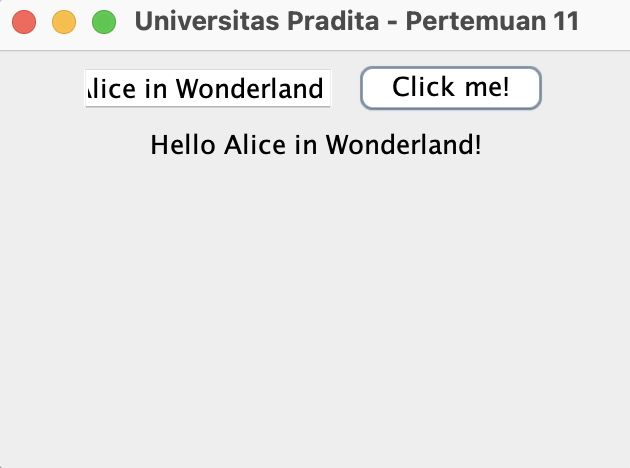
\includegraphics[width=0.8\textwidth]{assets/pertemuan11/simple_frame.png}
\end{center}


\textbf{Kode Java:}
\begin{lstlisting}[style=JavaStyle]
	package edu.pradita.p11;
	
	import java.awt.event.ActionEvent;
	import java.awt.event.ActionListener;
	import javax.swing.JButton;
	import javax.swing.JFrame;
	import javax.swing.JLabel;
	import javax.swing.JPanel;
	import javax.swing.JTextField;
	
	public class SimpleFrame extends JFrame {
		
		private JTextField textField;
		private JLabel label;
		
		public SimpleFrame() {
			setTitle("Simple Frame");
			setSize(300, 200);
			setDefaultCloseOperation(JFrame.EXIT_ON_CLOSE);
			setLocationRelativeTo(null);
			
			JPanel panel = new JPanel();
			getContentPane().add(panel);
			panel.setLayout(null);
			
			JLabel promptLabel = new JLabel("Enter your name:");
			promptLabel.setBounds(10, 20, 150, 25);
			panel.add(promptLabel);
			
			textField = new JTextField();
			textField.setBounds(10, 50, 160, 25);
			panel.add(textField);
			
			JButton button = new JButton("Say Hello");
			button.setBounds(10, 80, 160, 25);
			panel.add(button);
			
			label = new JLabel();
			label.setBounds(10, 110, 250, 25);
			panel.add(label);
			
			button.addActionListener(new ActionListener() {
				@Override
				public void actionPerformed(ActionEvent e) {
					String name = textField.getText();
					label.setText("Hello, " + name + "!");
				}
			});
		}
		
		public static void main(String[] args) {
			SimpleFrame frame = new SimpleFrame();
			frame.setVisible(true);
		}
	}
\end{lstlisting}

\subsection{Form dengan WindowBuilder}

\textbf{Kode:} \texttt{MyForm.java}

\textbf{Deskripsi:} Kode ini menciptakan formulir dengan beberapa komponen Swing, termasuk \texttt{JTextField}, \texttt{JSpinner}, dan \texttt{JButton}. Program ini juga menambahkan tombol yang memungkinkan pengguna untuk menambahkan tombol lain ke dalam formulir secara dinamis.

\textbf{Penjelasan Kode:}
\begin{itemize}
	\item \texttt{MyForm} adalah kelas yang membuat formulir dengan komponen GUI.
	\item \texttt{JTextField} digunakan untuk memasukkan teks, dan \texttt{JSpinner} untuk memilih nilai numerik.
	\item \texttt{JButton} digunakan untuk menyimpan data dan menambahkan tombol tambahan ke formulir.
	\item Metode \texttt{initialize()} mengatur layout dan menambahkan komponen ke formulir.
\end{itemize}

\textbf{Gambar:} \\
\begin{center}
	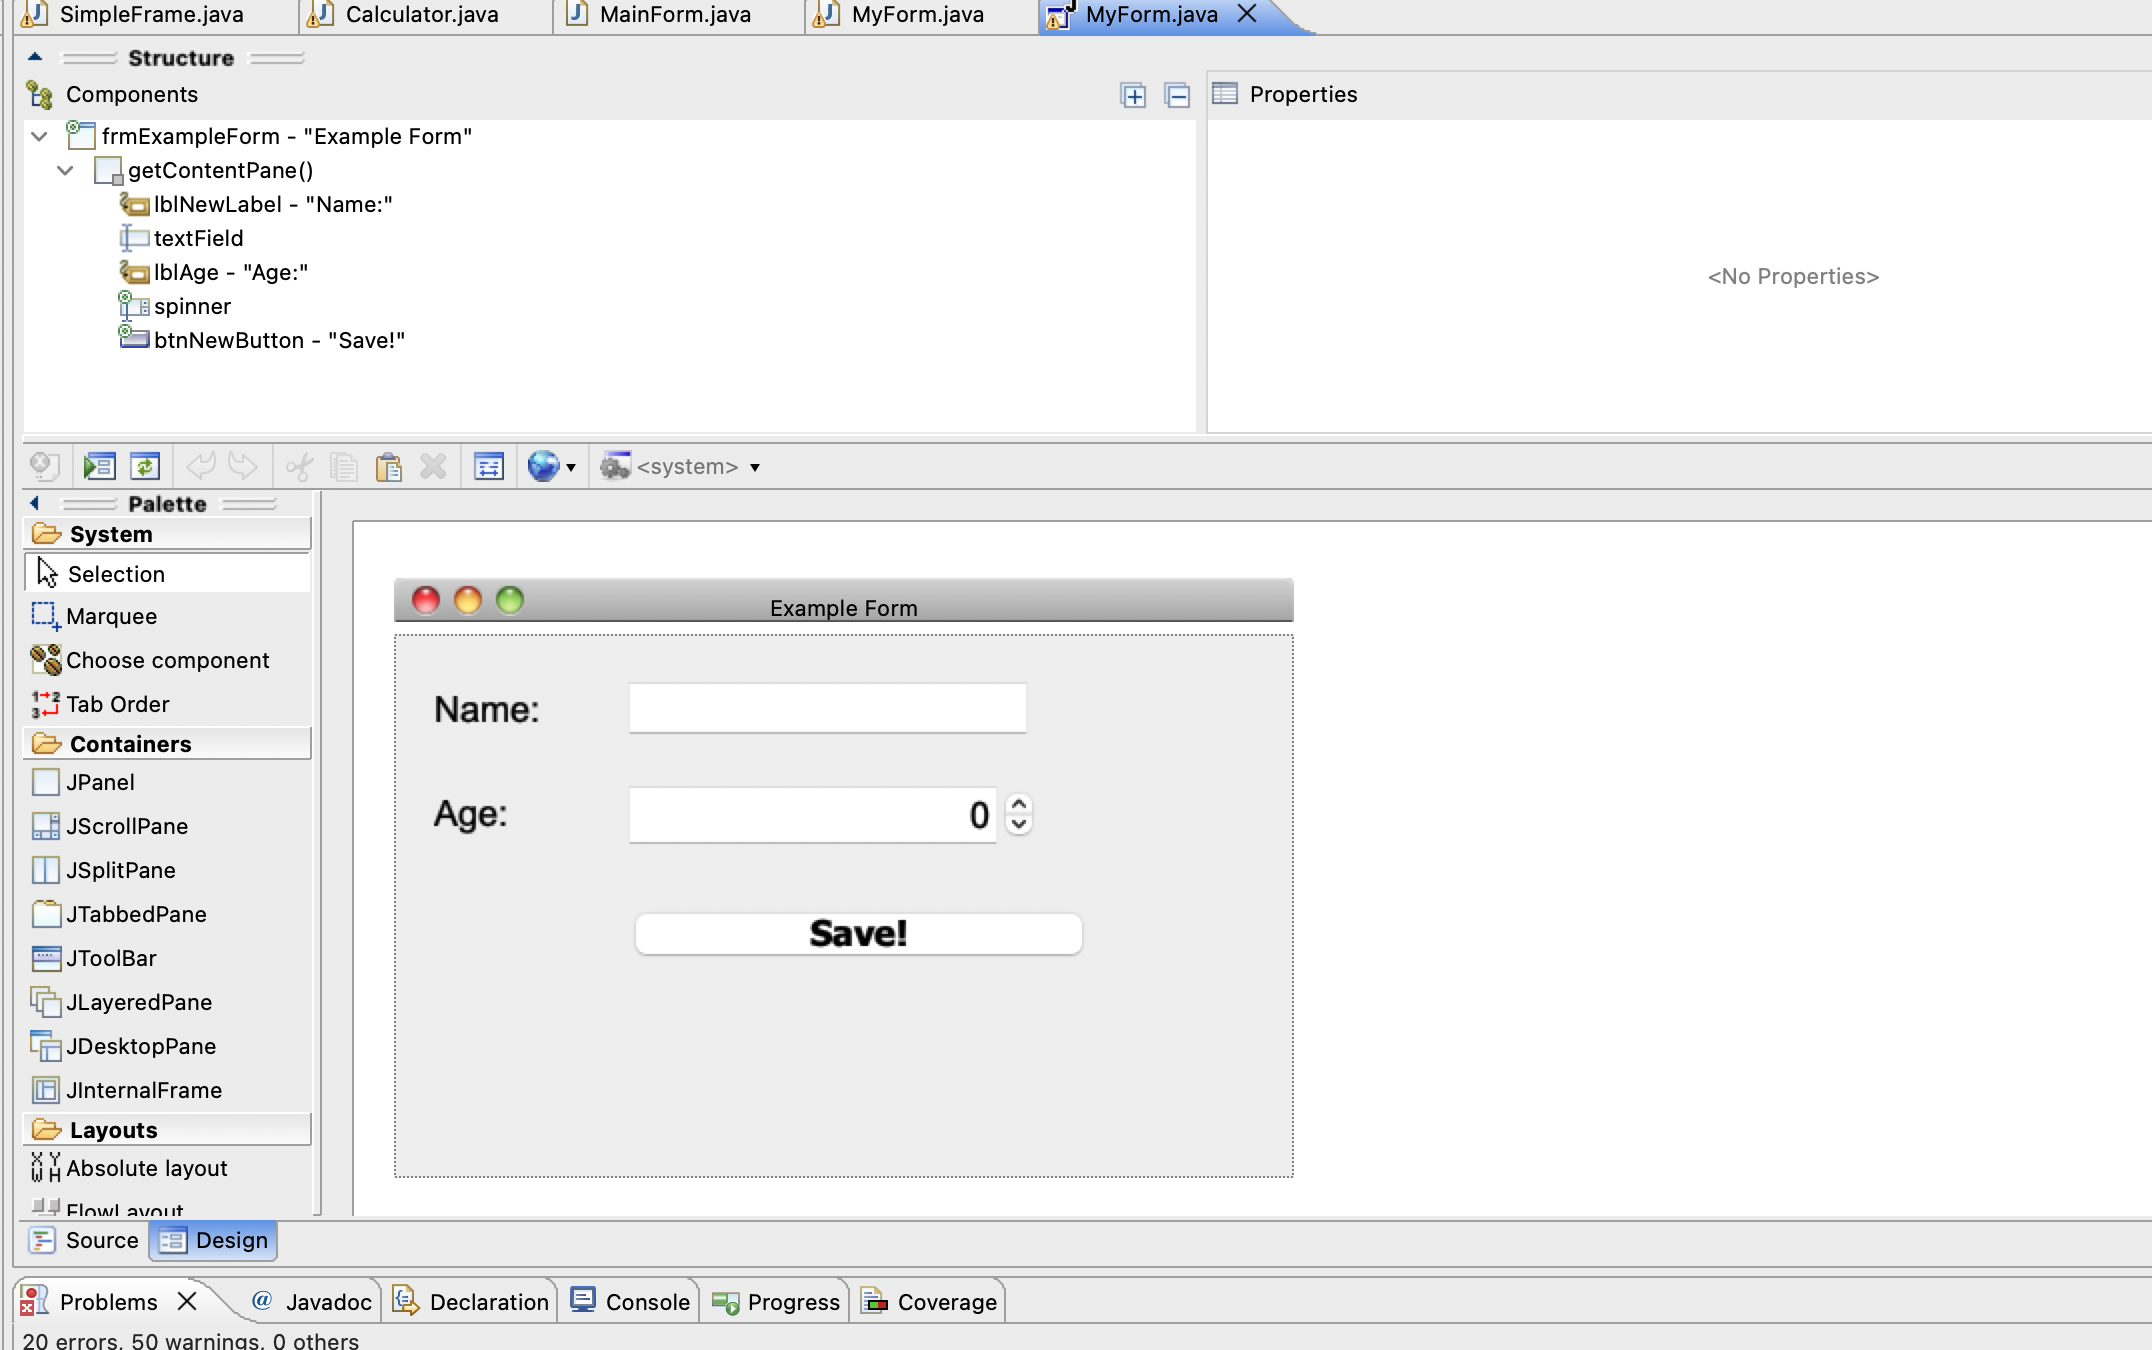
\includegraphics[width=0.8\textwidth]{assets/pertemuan11/myform_window_builder.png}
	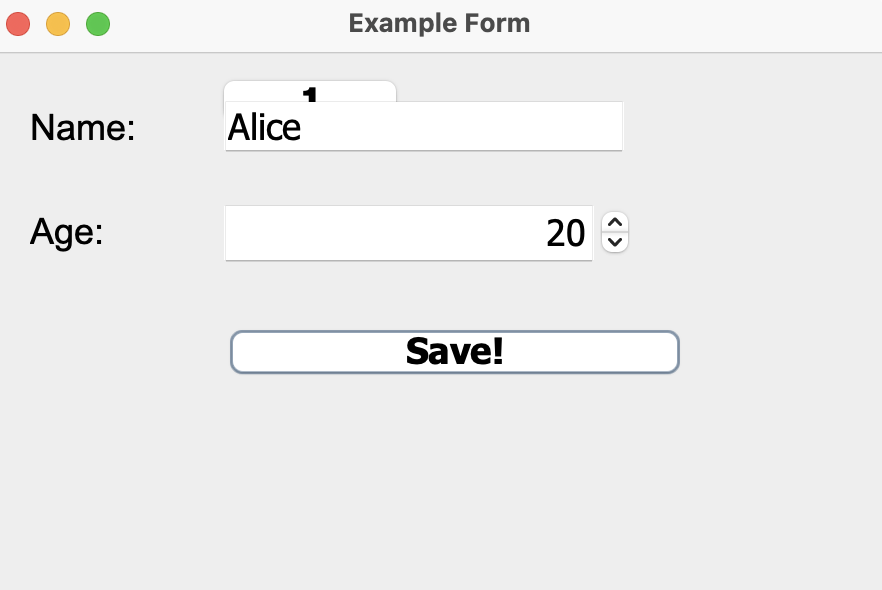
\includegraphics[width=0.8\textwidth]{assets/pertemuan11/myform.png}
	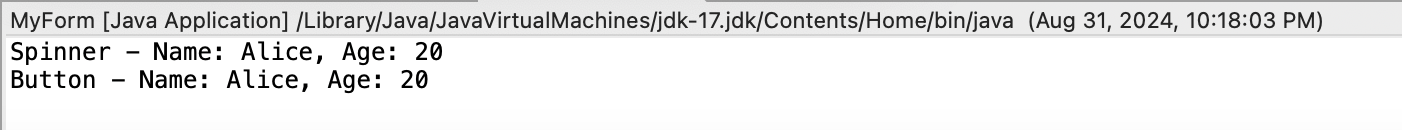
\includegraphics[width=0.8\textwidth]{assets/pertemuan11/myform_result.png}
\end{center}

\textbf{Kode Java:}
\begin{lstlisting}[style=JavaStyle]
	package edu.pradita.p11;
	
	import java.awt.EventQueue;
	import java.awt.Font;
	import java.awt.event.ActionEvent;
	import java.awt.event.ActionListener;
	import javax.swing.JButton;
	import javax.swing.JFrame;
	import javax.swing.JLabel;
	import javax.swing.JPanel;
	import javax.swing.JTextField;
	import javax.swing.JSpinner;
	import javax.swing.SpinnerNumberModel;
	
	public class MyForm extends JFrame {
		
		private JTextField nameField;
		private JSpinner ageSpinner;
		private JButton addButton;
		private JPanel panel;
		
		public MyForm() {
			initialize();
		}
		
		private void initialize() {
			setTitle("My Form");
			setBounds(100, 100, 450, 300);
			setDefaultCloseOperation(JFrame.EXIT_ON_CLOSE);
			panel = new JPanel();
			getContentPane().add(panel);
			panel.setLayout(null);
			
			JLabel nameLabel = new JLabel("Name:");
			nameLabel.setFont(new Font("Arial", Font.PLAIN, 14));
			nameLabel.setBounds(10, 20, 80, 25);
			panel.add(nameLabel);
			
			nameField = new JTextField();
			nameField.setBounds(100, 20, 165, 25);
			panel.add(nameField);
			
			JLabel ageLabel = new JLabel("Age:");
			ageLabel.setFont(new Font("Arial", Font.PLAIN, 14));
			ageLabel.setBounds(10, 50, 80, 25);
			panel.add(ageLabel);
			
			ageSpinner = new JSpinner(new SpinnerNumberModel(18, 0, 100, 1));
			ageSpinner.setBounds(100, 50, 50, 25);
			panel.add(ageSpinner);
			
			addButton = new JButton("Add");
			addButton.setBounds(10, 80, 80, 25);
			panel.add(addButton);
			
			addButton.addActionListener(new ActionListener() {
				@Override
				public void actionPerformed(ActionEvent e) {
					// Add action handling code here
				}
			});
			
			JButton addDynamicButton = new JButton("Add Dynamic Button");
			addDynamicButton.setBounds(10, 110, 200, 25);
			panel.add(addDynamicButton);
			
			addDynamicButton.addActionListener(new ActionListener() {
				@Override
				public void actionPerformed(ActionEvent e) {
					JButton dynamicButton = new JButton("Dynamic Button");
					dynamicButton.setBounds(10, 140 + (panel.getComponentCount() - 6) * 30, 200, 25);
					panel.add(dynamicButton);
					panel.revalidate();
					panel.repaint();
				}
			});
		}
		
		public static void main(String[] args) {
			EventQueue.invokeLater(new Runnable() {
				public void run() {
					try {
						MyForm frame = new MyForm();
						frame.setVisible(true);
					} catch (Exception e) {
						e.printStackTrace();
					}
				}
			});
		}
	}
\end{lstlisting}

\subsection{Kalkulator GUI}

\textbf{Kode:} \texttt{Calculator.java}

\textbf{Deskripsi:} Kode ini membuat aplikasi kalkulator sederhana menggunakan Swing di Java. Program ini terdiri dari beberapa komponen GUI seperti tombol angka, tombol operasi, dan layar tampilan.

\textbf{Penjelasan Kode:}
\begin{itemize}
	\item \texttt{Calculator} adalah kelas utama yang memperluas \texttt{JFrame} untuk membuat jendela GUI.
	\item \texttt{JPanel} digunakan untuk menyusun komponen dengan layout \texttt{BorderLayout} dan \texttt{GridLayout}.
	\item \texttt{JLabel} digunakan untuk menampilkan hasil kalkulasi.
	\item Tombol angka dibuat secara dinamis dalam sebuah loop dan ditambahkan ke panel tombol.
	\item Tombol \texttt{+} dan \texttt{=} ditambahkan untuk melakukan operasi penjumlahan dan menampilkan hasil.
	\item \texttt{calculate()} adalah metode untuk menghitung hasil operasi berdasarkan nilai yang disimpan dalam \texttt{accumulator}.
\end{itemize}

\textbf{Gambar:} \\
\begin{center}
	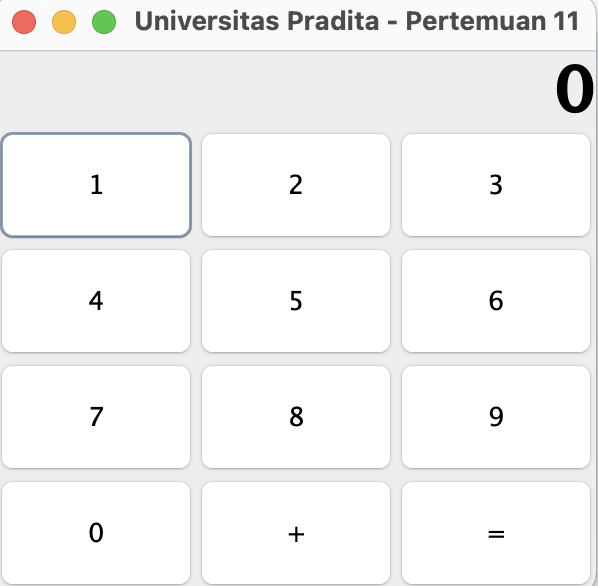
\includegraphics[width=0.5\textwidth]{assets/pertemuan11/calculator.png}
\end{center}

\textbf{Kode Java:}
\begin{lstlisting}[style=JavaStyle]
	package edu.pradita.p11;
	
	import java.awt.BorderLayout;
	import java.awt.Font;
	import java.awt.GridLayout;
	import java.awt.event.ActionEvent;
	import java.awt.event.ActionListener;
	import javax.swing.JButton;
	import javax.swing.JFrame;
	import javax.swing.JLabel;
	import javax.swing.JPanel;
	
	public class Calculator extends JFrame {
		
		private static final int FRAME_WIDTH = 300;
		private static final int FRAME_HEIGHT = 300;
		private static final int FONT_SIZE = 32;
		
		private Integer accumulator = null;
		private Integer value = 0;
		private String nextOperation = null;
		private boolean clearDisplay = false;
		
		public Calculator() {
			JPanel mainPanel = new JPanel();
			mainPanel.setLayout(new BorderLayout());
			this.add(mainPanel);
			
			JLabel display = new JLabel();
			display.setHorizontalAlignment(JLabel.RIGHT);
			display.setFont(new Font(display.getFont().getName(), Font.BOLD, 32));
			display.setText(String.valueOf(value));
			mainPanel.add(display, BorderLayout.NORTH);
			
			JPanel buttonPanel = new JPanel();
			buttonPanel.setLayout(new GridLayout(4, 3));
			mainPanel.add(buttonPanel, BorderLayout.CENTER);
			
			// Loop adding numeric button
			for (int i = 1; i <= 10; i++) {
				String valueText = (i < 10) ? valueText = String.valueOf(i) : "0";
				JButton button = new JButton();
				button.setText(valueText);
				buttonPanel.add(button);
				
				ActionListener numericButtonListener = new ActionListener() {
					@Override
					public void actionPerformed(ActionEvent e) {
						if (display.getText().equals("0")) {
							display.setText("" + button.getText());
						} else {
							if (clearDisplay) {
								display.setText("");
								clearDisplay = false;
							}
							display.setText(display.getText() + button.getText());
						}
						value = Integer.valueOf(display.getText());
					}
				};
				button.addActionListener(numericButtonListener);
			}
			
			// adding add button
			JButton button = new JButton();
			button.setText("+");
			buttonPanel.add(button);
			
			ActionListener addButtonListener = new ActionListener() {
				@Override
				public void actionPerformed(ActionEvent e) {
					nextOperation = "+";
					if (accumulator == null) {
						accumulator = Integer.valueOf(display.getText());
					} else {
						calculate();
						display.setText(String.valueOf(accumulator));
					}
					value = 0;
					clearDisplay = true;
				}
			};
			button.addActionListener(addButtonListener);
			
			// adding equal button
			JButton equalButton = new JButton();
			equalButton.setText("=");
			buttonPanel.add(equalButton);
			
			ActionListener equalButtonListener = new ActionListener() {
				@Override
				public void actionPerformed(ActionEvent e) {
					if (accumulator != null && nextOperation != null) {
						calculate();
						display.setText(String.valueOf(accumulator));
					}
					clearDisplay = true;
				}
			};
			equalButton.addActionListener(equalButtonListener);
			
			setSize(FRAME_WIDTH, FRAME_HEIGHT);
		}
		
		public void calculate() {
			if (nextOperation == "+") {
				accumulator = accumulator + value;
			}
		}
	}
\end{lstlisting}






\subsection{Main Form}

\textbf{Kode:} \texttt{MainForm.java}

\textbf{Deskripsi:} Kode ini membuat dua jendela GUI: satu untuk \texttt{SimpleFrame} dan satu untuk \texttt{Calculator}. \texttt{MainForm} adalah kelas utama yang menjalankan aplikasi dan menampilkan kedua jendela.

\textbf{Penjelasan Kode:}
\begin{itemize}
	\item \texttt{MainForm} adalah kelas utama dengan metode \texttt{main} yang membuat dan menampilkan jendela \texttt{SimpleFrame} dan \texttt{Calculator}.
	\item \texttt{frame.setLocationRelativeTo(null)} memastikan jendela ditempatkan di pusat layar.
	\item \texttt{setTitle}, \texttt{setDefaultCloseOperation}, dan \texttt{setVisible} digunakan untuk mengatur judul, operasi penutupan, dan visibilitas jendela.
\end{itemize}

\textbf{Gambar:} \\
\begin{center}
	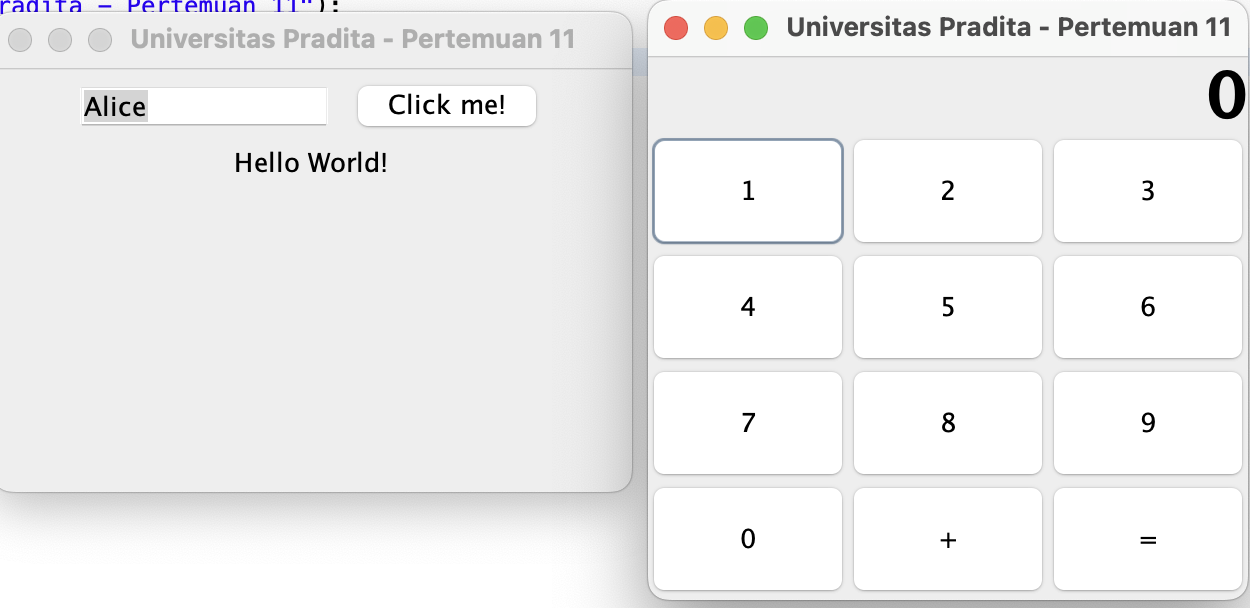
\includegraphics[width=0.8\textwidth]{assets/pertemuan11/main_form.png}
\end{center}

\textbf{Kode Java:}
\begin{lstlisting}[style=JavaStyle]
	package edu.pradita.p11;
	
	import javax.swing.JFrame;
	
	public class MainForm {
		public static void main(String[] args) {
			JFrame frame = new SimpleFrame();
			frame.setLocationRelativeTo(null); // put the frame at the centre
			frame.setTitle("Universitas Pradita - Pertemuan 11");
			frame.setDefaultCloseOperation(JFrame.EXIT_ON_CLOSE);
			frame.setVisible(true);
			
			JFrame calculator = new Calculator();
			calculator.setLocationRelativeTo(null); // put the frame at the centre
			calculator.setTitle("Universitas Pradita - Pertemuan 11");
			calculator.setDefaultCloseOperation(JFrame.EXIT_ON_CLOSE);
			calculator.setVisible(true);
		}
	}
\end{lstlisting}


\section{Latihan dan Contoh Kode: BMI Calculator}

Pada latihan ini, Anda akan membuat aplikasi GUI untuk menghitung Body Mass Index (BMI). Aplikasi ini harus memiliki inputan untuk berat badan (dalam kilogram) dan tinggi badan (dalam meter). Setelah pengguna memasukkan data dan menekan tombol “Hitung”, BMI akan ditampilkan di layar.

\textbf{Instruksi:}
\begin{enumerate}
	\item Buatlah GUI menggunakan WindowBuilder di Eclipse.
	\item Buatlah inputan untuk berat badan (dalam kilogram) dan tinggi badan (dalam meter).
	\item Tambahkan tombol “Hitung” yang akan menghitung BMI berdasarkan inputan pengguna.
	\item Tampilkan hasil BMI setelah tombol ditekan.
\end{enumerate}


\textbf{Gambar:} \\
\begin{center}
	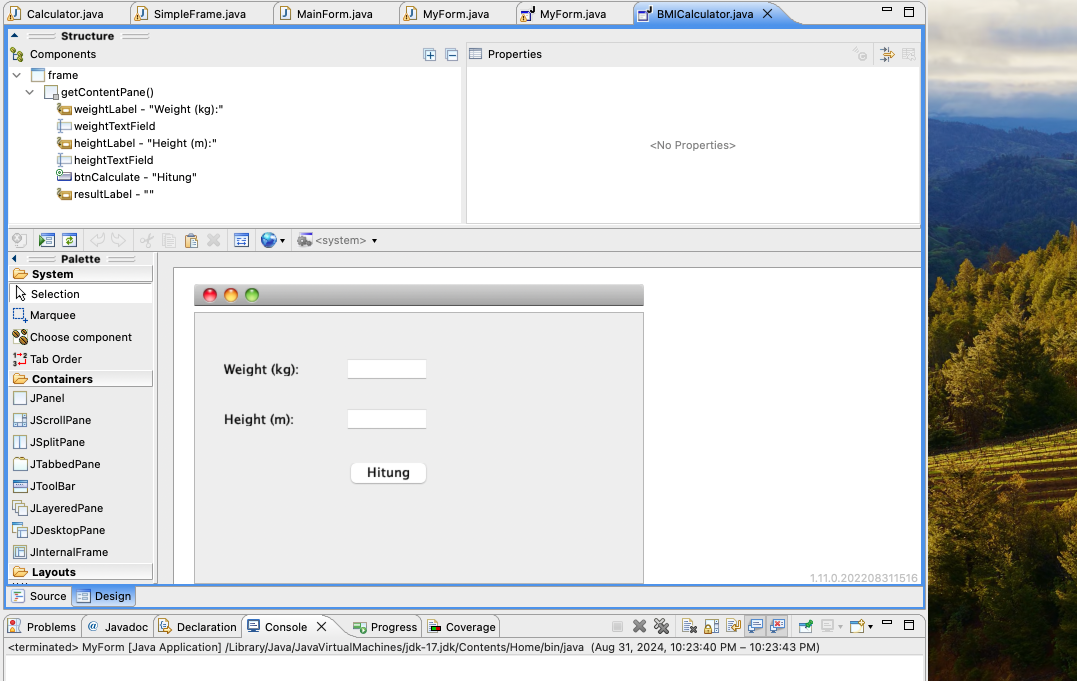
\includegraphics[width=0.8\textwidth]{assets/pertemuan11/bmicalculator_window_builder.png}
	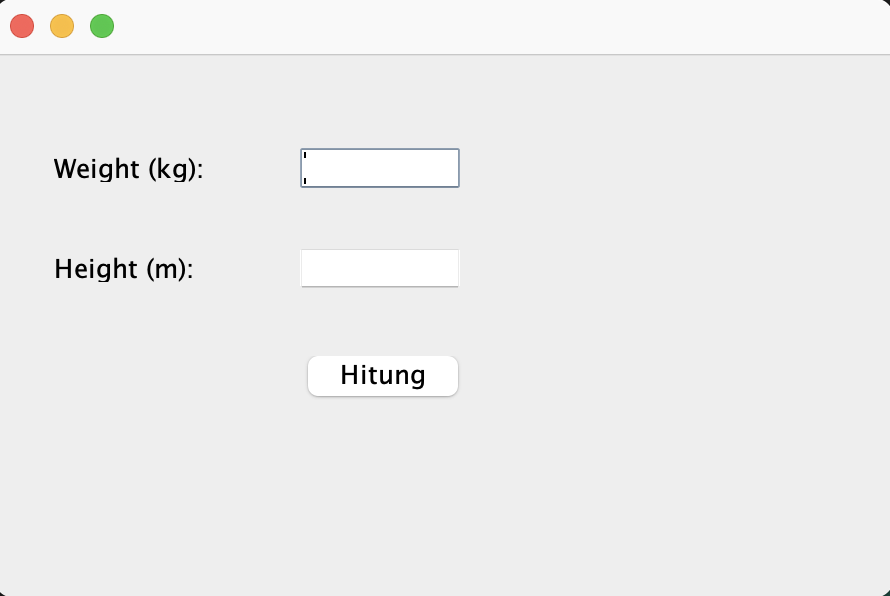
\includegraphics[width=0.8\textwidth]{assets/pertemuan11/bmicalculator.png}
\end{center}


\textbf{Kode Java:}

\begin{lstlisting}[style=JavaStyle]
	import java.awt.EventQueue;
	import javax.swing.JFrame;
	import javax.swing.JLabel;
	import javax.swing.JTextField;
	import javax.swing.JButton;
	import java.awt.event.ActionListener;
	import java.awt.event.ActionEvent;
	
	public class BMICalculator {
		
		private JFrame frame;
		private JTextField weightTextField;
		private JTextField heightTextField;
		private JLabel resultLabel;
		
		/**
		* Launch the application.
		*/
		public static void main(String[] args) {
			EventQueue.invokeLater(new Runnable() {
				public void run() {
					try {
						BMICalculator window = new BMICalculator();
						window.frame.setVisible(true);
					} catch (Exception e) {
						e.printStackTrace();
					}
				}
			});
		}
		
		/**
		* Create the application.
		*/
		public BMICalculator() {
			initialize();
		}
		
		/**
		* Initialize the contents of the frame.
		*/
		private void initialize() {
			frame = new JFrame();
			frame.setBounds(100, 100, 450, 300);
			frame.setDefaultCloseOperation(JFrame.EXIT_ON_CLOSE);
			frame.getContentPane().setLayout(null);
			
			JLabel weightLabel = new JLabel("Weight (kg):");
			weightLabel.setBounds(30, 50, 100, 14);
			frame.getContentPane().add(weightLabel);
			
			weightTextField = new JTextField();
			weightTextField.setBounds(150, 47, 86, 20);
			frame.getContentPane().add(weightTextField);
			weightTextField.setColumns(10);
			
			JLabel heightLabel = new JLabel("Height (m):");
			heightLabel.setBounds(30, 100, 100, 14);
			frame.getContentPane().add(heightLabel);
			
			heightTextField = new JTextField();
			heightTextField.setBounds(150, 97, 86, 20);
			frame.getContentPane().add(heightTextField);
			heightTextField.setColumns(10);
			
			JButton btnCalculate = new JButton("Hitung");
			btnCalculate.addActionListener(new ActionListener() {
				public void actionPerformed(ActionEvent e) {
					double weight = Double.parseDouble(weightTextField.getText());
					double height = Double.parseDouble(heightTextField.getText());
					double bmi = weight / (height * height);
					resultLabel.setText(String.format("Your BMI is: %.2f", bmi));
				}
			});
			btnCalculate.setBounds(150, 150, 89, 23);
			frame.getContentPane().add(btnCalculate);
			
			resultLabel = new JLabel("");
			resultLabel.setBounds(150, 200, 200, 14);
			frame.getContentPane().add(resultLabel);
		}
	}
\end{lstlisting}


\section{Soal}

Berikut adalah instruksi untuk dua proyek yang akan membantu memahami penggunaan \textit{Java Swing} dalam membangun aplikasi sederhana.

\subsection*{Proyek 1: Permainan Tic-Tac-Toe}
\textbf{Tujuan}: Mengembangkan permainan Tic-Tac-Toe interaktif sederhana menggunakan Java Swing untuk dua pemain.

\textbf{Instruksi}:
\begin{enumerate}
	\item \textbf{Atur GUI}:
	\begin{itemize}
		\item Buat papan permainan 3x3 menggunakan \texttt{JPanel} dengan \texttt{GridLayout} untuk papan Tic-Tac-Toe.
		\item Tambahkan sembilan \texttt{JButton} dalam grid untuk mewakili kotak-kotak tempat pemain akan menempatkan simbol mereka (X atau O).
	\end{itemize}
	
	\item \textbf{Logika Permainan}:
	\begin{itemize}
		\item Terapkan logika pergantian giliran agar permainan bergiliran antara dua pemain (Pemain X dan Pemain O).
		\item Gunakan variabel internal, seperti \texttt{boolean isXTurn}, untuk melacak giliran siapa saat ini. Inisialisasi dengan \texttt{true} (giliran Pemain X).
	\end{itemize}
	
	\item \textbf{Aksi Klik Tombol}:
	\begin{itemize}
		\item Tambahkan \texttt{ActionListener} ke masing-masing tombol. Ketika pemain mengklik tombol, periksa apakah kotak kosong.
		\item Jika kosong, perbarui tombol dengan simbol pemain saat ini (X atau O), lalu ubah giliran dengan memperbarui \texttt{isXTurn}.
		\item Nonaktifkan tombol setelah diklik untuk mencegah perubahan lebih lanjut.
	\end{itemize}
	
	\item \textbf{Menentukan Pemenang}:
	\begin{itemize}
		\item Periksa pemenang setelah setiap gerakan dengan memeriksa label tombol di setiap baris, kolom, dan diagonal.
		\item Jika seorang pemain memiliki tiga simbol berturut-turut, tampilkan dialog pesan (misalnya, \texttt{JOptionPane.showMessageDialog}) yang menyatakan pemenang.
		\item Jika semua kotak terisi tanpa pemenang, tampilkan pesan yang menyatakan seri.
	\end{itemize}
	
	\item \textbf{Opsi Reset}:
	\begin{itemize}
		\item Tambahkan tombol "Permainan Baru" atau "Reset" untuk memulai permainan baru.
		\item Atur ulang semua tombol menjadi kosong dan aktifkan kembali untuk permainan baru. Set \texttt{isXTurn} kembali ke \texttt{true} untuk memulai dengan Pemain X.
	\end{itemize}
	
	\item \textbf{Penanganan Kesalahan}:
	\begin{itemize}
		\item Pastikan tindakan tidak valid dicegah, seperti mengklik kotak yang sudah berisi simbol.
		\item Tangani setiap pengecualian secara tepat, memberikan umpan balik yang bermanfaat jika diperlukan.
	\end{itemize}
\end{enumerate}

\textbf{Hasil Akhir}: Program permainan Tic-Tac-Toe yang berfungsi, bergiliran, memeriksa pemenang atau seri, dan dapat diatur ulang.

\subsection*{Proyek 2: Aplikasi Daftar Tugas}
\textbf{Tujuan}: Membangun aplikasi Daftar Tugas yang memungkinkan pengguna menambah, menandai, dan menghapus tugas.

\textbf{Instruksi}:
\begin{enumerate}
	\item \textbf{Atur GUI}:
	\begin{itemize}
		\item Buat \texttt{JFrame} utama untuk jendela aplikasi.
		\item Tambahkan \texttt{JTextField} di bagian atas untuk mengetik tugas yang ingin ditambahkan.
		\item Tambahkan tombol "Tambahkan Tugas" di samping kolom teks untuk menambah tugas ke daftar.
		\item Gunakan komponen \texttt{JList} untuk menampilkan daftar tugas. Atur model daftar dengan menggunakan (\texttt{DefaultListModel<String>}) untuk menambah dan menghapus tugas secara dinamis.
	\end{itemize}
	
	\item \textbf{Menambah Tugas}:
	\begin{itemize}
		\item Ketika pengguna mengetik tugas dan menekan tombol "Tambahkan Tugas", tambahkan tugas ke dalam \texttt{JList}.
		\item Kosongkan kolom teks setelah menambahkan tugas untuk memudahkan penambahan berikutnya.
	\end{itemize}
	
	\item \textbf{Menandai Tugas sebagai Selesai}:
	\begin{itemize}
		\item Tambahkan tombol "Tandai Selesai" yang memungkinkan pengguna menandai tugas yang dipilih sebagai selesai.
		\item Ketika pengguna memilih tugas di \texttt{JList} dan menekan "Tandai Selesai", perbarui tampilan tugas (misalnya, tambahkan tanda "(Selesai)" atau ubah warnanya).
	\end{itemize}
	
	\item \textbf{Menghapus Tugas}:
	\begin{itemize}
		\item Tambahkan tombol "Hapus Tugas" yang menghapus tugas yang dipilih dari daftar ketika diklik.
		\item Konfirmasi penghapusan dengan dialog (\texttt{JOptionPane.showConfirmDialog}) untuk mencegah penghapusan tidak sengaja.
	\end{itemize}
	
	\item \textbf{Opsi Hapus Semua}:
	\begin{itemize}
		\item Secara opsional, tambahkan tombol "Hapus Semua" yang menghapus semua tugas dari daftar setelah konfirmasi dari pengguna.
	\end{itemize}
	
	\item \textbf{Penanganan Kesalahan}:
	\begin{itemize}
		\item Pastikan tindakan seperti menandai atau menghapus hanya memengaruhi tugas saat satu tugas dipilih. Tampilkan pesan kesalahan jika tidak ada tugas yang dipilih.
	\end{itemize}
\end{enumerate}

\textbf{Hasil Akhir}: Program Aplikasi Daftar Tugas yang dapat menambah, menandai selesai, dan menghapus tugas dengan tampilan yang jelas dan mudah digunakan.



